\documentclass{beamer}
\usepackage[unilu,en]{collegeBeamer}
\usepackage[backend=biber]{biblatex}
\usepackage[usenames,dvipsnames]{xcolor}
\setbeamertemplate{footline}[frame number]
\usepackage{graphicx}
\usepackage{tikz}
\usetikzlibrary{calc, arrows.meta, intersections, patterns, positioning, shapes.misc, shapes.geometric, fadings, through, decorations.pathreplacing}
\usepackage{etoolbox}

\addbibresource{references.bib}

% meta-data
\title{GraphSAGE}
\subtitle{Inductive Representation Learning\\on Large Graphs}
\author{Thomas Gantz\\Alberto Finardi\\Tommaso Crippa\\Jan Marxen}
\date{\today}
\themecolor{50,50,50}

% document body
\begin{document}

\maketitle

%-----------------------------------------------------------------------
\section{Introduction}
%-----------------------------------------------------------------------

\begin{frame}{Graph Prediction Tasks}
    \begin{columns}
        \begin{column}{0.55\textwidth}
            \textbf{Primary focus:} Node-level prediction — predict properties of individual nodes (classification, regression).
            
            \vspace{10pt}
            \begin{itemize}
                \item \textbf{Node-level (focus):} Predict node attributes or labels using features and neighbor information.
                \item \textbf{Edge-level:} Predict relationships between node pairs (link prediction, edge classification).
                \item \textbf{Graph-level:} Predict properties of whole graphs (e.g., molecule properties).
            \end{itemize}
        \end{column}
        \begin{column}{0.42\textwidth}
            \centering
            \includegraphics[width=1.2\textwidth]{img/gnn_intro_node_level_task.png}
        \end{column}
    \end{columns}
\end{frame}

\begin{frame}{What is a Graph Neural Network?}

    \vspace{4pt}
    \textbf{A learnable transformation} on graph attributes that:
    \begin{itemize}
        \item Updates node/edge/graph features using \textbf{neural networks}
        \item \textbf{Respects graph structure} by aggregating information from neighbors
        \item Is \textbf{permutation invariant} (order of nodes doesn't matter)
    \end{itemize}
    
    \vspace{5pt}
    \centering
    \includegraphics[width=0.75\textwidth]{img/gnn_intro_whatisgnn.png}
\end{frame}

\begin{frame}{Message Passing: The Core Idea}
    \textbf{Three steps repeated at each layer:}
    \begin{enumerate}
        \item \textbf{Gather:} Collect embeddings from neighboring nodes
        \item \textbf{Aggregate:} Combine neighbors' info (sum / mean / max)
        \item \textbf{Update:} Apply learned transform using the aggregated vector
    \end{enumerate}
    
    \vspace{6pt}
    \centering
    \includegraphics[width=0.85\textwidth]{img/gnn_intro_message_passing.png}
\end{frame}

\begin{frame}{Message Passing: Notation}
    \begin{block}{Message Passing Equation}
        \centering
        $h_v^{(k)} = \sigma\left( W \cdot \left[ h_v^{(k-1)} \, , \, \mathrm{AGG}\left(\{ h_u : u \in N(v) \}\right) \right] \right)$
    \end{block}
    
    \vspace{4pt}
    \begin{columns}
        \begin{column}{0.48\textwidth}
            \small
            \begin{itemize}
                \item $h_v^{(k)}$ — Node $v$ repr. at layer $k$
                \item $h_u$ — Neighbor node $u$ repr.
                \item $N(v)$ — Neighbors of $v$
                \item $k$ — Layer index (hops)
            \end{itemize}
        \end{column}
        \begin{column}{0.48\textwidth}
            \small
            \begin{itemize}
                \item $\mathrm{AGG}(\cdot)$ — Aggregator (mean, sum, max)
                \item $W$ — Learnable weight matrix
                \item $\sigma$ — Activation (ReLU, tanh)
            \end{itemize}
        \end{column}
    \end{columns}
\end{frame}

\begin{frame}{Before GraphSAGE: The Problem}
    \textit{Let's audit the limitations of existing approaches...}
    
    \vspace{12pt}
    \begin{itemize}
        \item \textbf{DeepWalk / node2vec:} Transductive: embed every node; new nodes need full retraining.\\
              \hspace{1em}{\small \textcolor{gray}{$\triangleright$ Not GNNs — random-walk based embeddings, no message passing}}
        \item \textbf{GCNs:} Often require access to the full graph during training/inference; can be costly to scale.\\
              \hspace{1em}{\small \textcolor{gray}{$\triangleright$ GNNs — but transductive: fixed node set at training}}
        \item \textbf{Result:} No compact parametric function to generate embeddings for unseen nodes.
    \end{itemize}
    
    \vspace{12pt}
    \textit{This motivates GraphSAGE's key insight...}
\end{frame}

%-----------------------------------------------------------------------
\section{The Key Insight}
%-----------------------------------------------------------------------

\begin{frame}{The Key Insight}
    \centering
    \vspace{5pt}
    
    {\Large \textbf{Don't learn embeddings for each node...}}
    
    \vspace{10pt}
    
    {\Large \textcolor{orange}{\textbf{Learn a FUNCTION that generates embeddings}}}
    
    \vspace{8pt}
    
    \textit{By sampling \& aggregating neighborhood features}
    
    \vspace{8pt}
    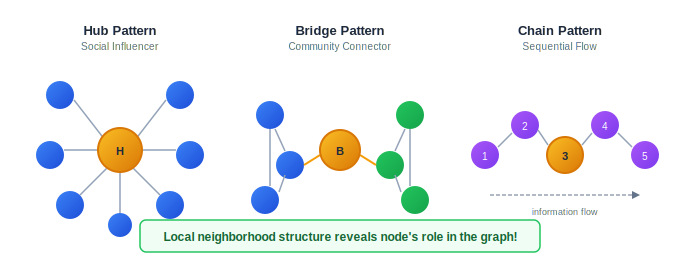
\includegraphics[width=0.65\textwidth]{img/graphs_examples_light.png}
\end{frame}

%-----------------------------------------------------------------------
\section{GraphSAGE Framework}
%-----------------------------------------------------------------------

\begin{frame}{GraphSAGE: Inductive Framework}
    \textbf{Core Principle:} Sample + Aggregate
    
    \vspace{10pt}
    \begin{itemize}
        \item Learn \textbf{aggregator functions} (not node embeddings)
        \item For any node $v$: \textbf{sample neighbors, aggregate their features}
        \item Pass through learned neural networks
        \item \textbf{Inference:} Apply same function to unseen nodes
    \end{itemize}
    
    \vspace{10pt}
    \centering
    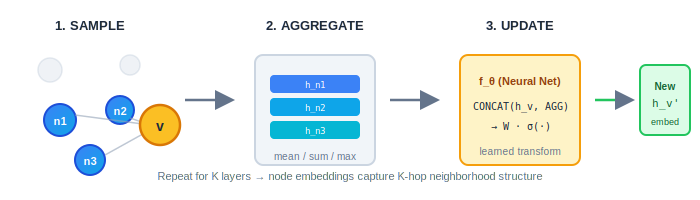
\includegraphics[width=0.95\textwidth]{img/graphsage_sample_aggregate_light.png}
\end{frame}

%-----------------------------------------------------------------------
\section{Implementation}
%-----------------------------------------------------------------------

\begin{frame}{System Architecture Overview}
    \textbf{Dataset:} ogbn-products (Amazon co-purchase network)
    \begin{itemize}
        \item 2.4M nodes (products), 61M edges, 47 classes
        \item 8\% train / 2\% val / 90\% test split
    \end{itemize}

    \vspace{8pt}
    \textbf{Training Environment:}
    \begin{itemize}
        \item \textbf{HPC Cluster:} MeluXina (Luxembourg National Supercomputer)
        \item \textbf{GPUs:} Up to 4x NVIDIA A100 (40GB) per node
        \item \textbf{Framework:} PyTorch 2.1.2 + PyTorch Geometric
        \item \textbf{Containerization:} Apptainer/Singularity for reproducibility
    \end{itemize}

    \vspace{8pt}
    \textbf{Model Architecture:}
    \begin{itemize}
        \item 5-layer GraphSAGE (SAGEConv + LayerNorm + ReLU)
        \item Hidden dimension: 256, Dropout: 0.5
    \end{itemize}
\end{frame}

\begin{frame}{System Architecture Diagram}
    \centering
    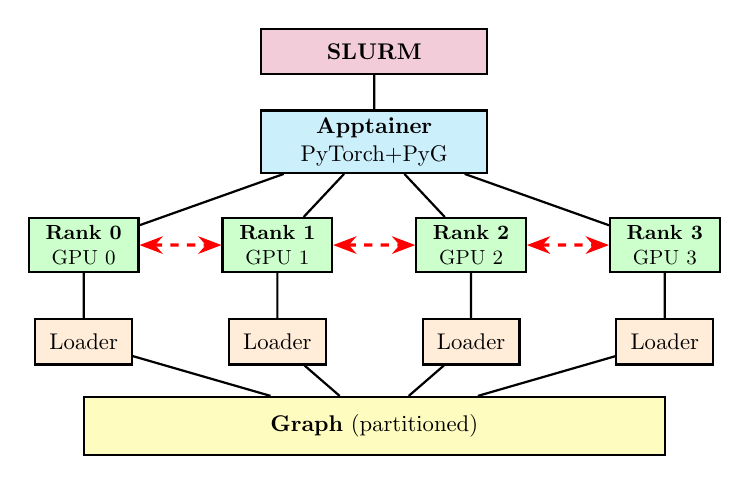
\begin{tikzpicture}[scale=0.82, every node/.style={transform shape}]

    % Styles
    \tikzset{
        boxstyle/.style={rectangle, draw, thick, minimum height=0.7cm, align=center},
        gpu/.style={boxstyle, fill=green!20, minimum width=1.7cm, font=\small},
        loader/.style={boxstyle, fill=orange!15, minimum width=1.5cm},
        graphbox/.style={boxstyle, fill=yellow!25, minimum width=9cm, minimum height=0.9cm},
        arrow/.style={-, >=Stealth, thick},
        redarrow/.style={<->, >=Stealth, very thick, red, dashed}
    }

    % Top layers
    \node[boxstyle, fill=purple!20, minimum width=3.5cm] (slurm) at (0, 5.2) {\textbf{SLURM}};
    \node[boxstyle, fill=cyan!20, minimum width=3.5cm] (container) at (0, 3.8) {\textbf{Apptainer}\\PyTorch+PyG};

    % GPU ranks
    \node[gpu] (r0) at (-4.5, 2.2) {\textbf{Rank 0}\\GPU 0};
    \node[gpu] (r1) at (-1.5, 2.2) {\textbf{Rank 1}\\GPU 1};
    \node[gpu] (r2) at (1.5, 2.2) {\textbf{Rank 2}\\GPU 2};
    \node[gpu] (r3) at (4.5, 2.2) {\textbf{Rank 3}\\GPU 3};

    % NCCL
    \draw[redarrow] (r0) -- (r1);
    \draw[redarrow] (r1) -- (r2);
    \draw[redarrow] (r2) -- (r3);

    % Loaders
    \node[loader] (l0) at (-4.5, 0.7) {Loader};
    \node[loader] (l1) at (-1.5, 0.7) {Loader};
    \node[loader] (l2) at (1.5, 0.7) {Loader};
    \node[loader] (l3) at (4.5, 0.7) {Loader};

    % Graph data
    \node[graphbox] (gdata) at (0, -0.6) {\textbf{Graph} (partitioned)};

    % Arrows
    \draw[arrow] (slurm) -- (container);
    \foreach \r in {r0,r1,r2,r3} {
        \draw[arrow] (container) -- (\r);
    }
    \foreach \i in {0,1,2,3} {
        \draw[arrow] (r\i) -- (l\i);
        \draw[arrow] (gdata) -- (l\i);
    }

    \end{tikzpicture}

    \vspace{3pt}
    {\footnotesize Multi-GPU DDP: data partitioned across 4 GPUs, gradients synced via NCCL}
\end{frame}

\begin{frame}{Execution Model: Distributed Data Parallel}

    \textbf{Process Initialization:}
    \begin{itemize}
        \item SLURM launches 4 processes (1 per GPU) on single node
        \item Each process: independent Python interpreter + CUDA context
        \item NCCL backend for GPU-to-GPU communication (InfiniBand)
    \end{itemize}

    \vspace{8pt}
    \textbf{Data Distribution:}
    \begin{itemize}
        \item Training set (250k nodes) partitioned: 62.5k per rank
        \item No overlap between ranks \textrightarrow\ each processes unique subset
        \item Each rank has independent NeighborLoader for k-hop sampling
    \end{itemize}

    \vspace{8pt}
    \textbf{Gradient Synchronization:}
    \begin{itemize}
        \item DDP automatically wraps model: synchronizes gradients after backward()
        \item All-reduce operation: averages gradients across all GPUs
        \item Learning rate scaled linearly: $\text{lr}_{\text{eff}} = \text{lr}_{\text{base}} \times N_{\text{GPUs}}$
    \end{itemize}
\end{frame}

\begin{frame}{Execution Model: Training Workflow}
    \begin{enumerate}
        \item \textbf{Data Loading (Parallel)}:
        \begin{itemize}
            \item Each rank: 4-8 worker processes prefetch batches
            \item NeighborLoader samples k-hop subgraphs
            \item Pinned memory \textrightarrow\ GPU transfer (non-blocking)
        \end{itemize}

        \vspace{4pt}
        \item \textbf{Forward + Backward (Parallel)}:
        \begin{itemize}
            \item Each GPU: processes batch independently
            \item 5-layer message passing: aggregate \textrightarrow\ transform \textrightarrow\ activate
            \item Compute loss (cross-entropy), backpropagate gradients
        \end{itemize}

        \vspace{4pt}
        \item \textbf{Gradient Synchronization}:
        \begin{itemize}
            \item DDP all-reduce: average gradients across 4 GPUs (NCCL)
            \item Optimizer step with synchronized gradients
        \end{itemize}

        \vspace{4pt}
        \item \textbf{Evaluation (Rank 0 Only)}:
        \begin{itemize}
            \item Every 5 epochs: validation accuracy on full validation set
            \item Checkpoint best model, early stopping (patience = 10)
        \end{itemize}
    \end{enumerate}
\end{frame}

\begin{frame}{Code Structure \& Containerization}
    \textbf{Main Python Scripts:}
    \begin{itemize}
        \item \texttt{train\_graphsage.py} — Single-GPU training baseline
        \item \texttt{train\_graphsage\_ddp.py} — Multi-GPU DDP training (enhanced)
        \item \texttt{plot\_batch.py} — Batch size benchmarking analysis
        \item \texttt{plot\_neighbor.py} — Neighbor sampling strategy analysis
    \end{itemize}

    \vspace{8pt}
    \textbf{Apptainer Container:}
    \begin{itemize}
        \item \textbf{Base:} \texttt{pytorch/pytorch:2.1.2-cuda12.1-cudnn8-runtime}
        \item \textbf{Dependencies:} PyTorch Geometric, pyg-lib, OGB, torch-scatter/sparse
        \item \textbf{Why containerize?}
        \begin{itemize}
            \item Complex dependency graph (CUDA-compiled extensions)
            \item Reproducibility across HPC environments
            \item Avoid version conflicts on shared cluster
        \end{itemize}
    \end{itemize}
\end{frame}

\begin{frame}{Why HPC and Parallelism?}
    \textbf{1. Scale of the Problem:}
    \begin{itemize}
        \item Dataset cannot fit in single GPU
        \item Neighbor sampling: Each batch node samples 5-hop neighborhoods
        \item Fanout [15,10,10,10,10] $\rightarrow$ exponential growth: $\sim$150k neighbors per seed node
        \item Batch 128 nodes $\times$ 150k expansion = 19.2M nodes per batch
    \end{itemize}

    \vspace{8pt}
    \textbf{2. Memory Bottleneck:}
    \begin{itemize}
        \item Model parameters: only $\sim$8 MB
        \item Sampled subgraphs + intermediate activations: \textbf{30-40 GB} per batch
        \item Single GPU (40 GB) cannot handle large batches $\rightarrow$ slow training
    \end{itemize}

    \vspace{8pt}
    \textbf{3. Solution: Multi-GPU Parallelism}
    \begin{itemize}
        \item Split data across 4 GPUs $\rightarrow$ 4x memory capacity
        \item Effective batch size: 2048 nodes (faster convergence)
        \item Training time: \textbf{hours instead of days}
    \end{itemize}
\end{frame}

%-----------------------------------------------------------------------
\section{Hyperparameters}
%-----------------------------------------------------------------------

\begin{frame}{Hyperparameters}
    \centering
    \vspace{30pt}
    {\Large \textit{Hyperparameter tuning details coming soon...}}
    \vspace{30pt}
\end{frame}

%-----------------------------------------------------------------------
\section{Results}
%-----------------------------------------------------------------------

\begin{frame}{Results}
    \centering
    \vspace{30pt}
    {\Large \textit{Experimental results coming soon...}}
    \vspace{30pt}
\end{frame}

%-----------------------------------------------------------------------
\QApage

\bibliographpage

\end{document}
